
\chapter{METODOLOGÍA, CONSIDERACIONES Y SUPUESTOS.} %(((
\begin{itemize}
	\item El enfoque de ingresos no fue utilizado, ya que no se pudo establecer un nivel de ingresos específico para el equipo valuado.
	\item Para calcular la depreciación física se utilizó la metodología del análisis de edad efectiva y vida útil remanente, que se basa en establecer la edad cronológica del equipo ajustada por las reconstrucciones y mejoras que haya recibido el equipo y establecer cuanto tiempo más se espera que el equipo siga trabajando. 
	Con base a dichas estimaciones, se establece el porcentaje de vida transcurrido del equipo y ese factor se utiliza para afectar el precio de un bien equivalente nuevo.
\item Este tipo de equipo no presenta cambios significativos en los modelos valuados, por lo que la obsolescencia técnico funcional es nula.
\item Los equipos se encuentran desinstalados y fuera de operación, por lo tanto, no fue posible identificar la contaminación que generan los equipos, por lo que no se consideró depreciación por este concepto. 
\item No se incluyeron inventarios de ningún tipo, ni cualquier otro activo circulante o intangible, así como tampoco permisos, derechos, cuotas de contratación, etc., necesarios para la obtención de los diversos servicios de tipo operativo tales como: agua, energía eléctrica y similares, etc., así como tampoco el impuesto al valor agregado.
\item Obsolescencia económica. \\ 
El factor para calcular la obsolescencia económica, según el sector y clase de actividad; 311910 Elaboración de botanas, se tomó directamente del promedio de las publicaciones que emite el INEGI denominadas "Encuesta mensual de la industria manufacturera", considerando como último dato el correspondiente al mes de mayo de 2024.
\end{itemize}
\begin{figure}[hbtp!]
	\centering
	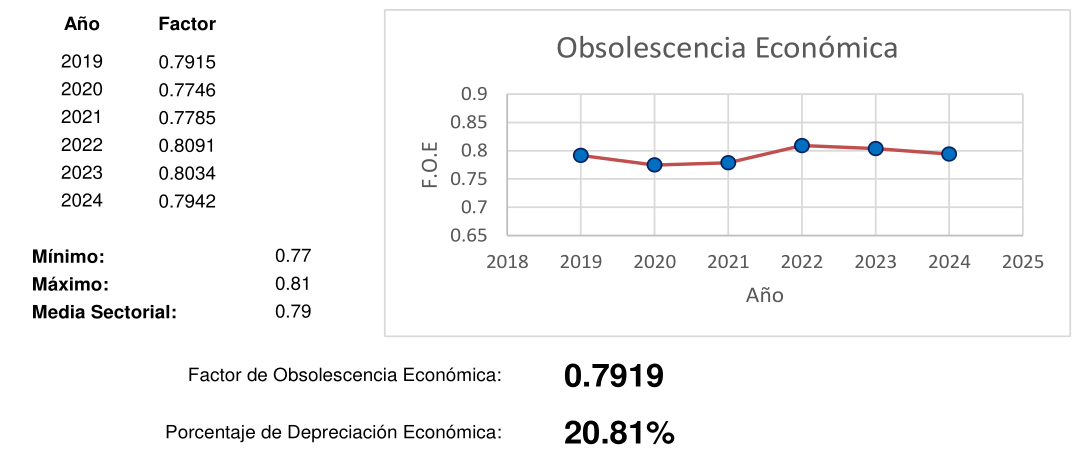
\includegraphics[width= \linewidth]{../0.imagenes/CAP_6/1}
	
\includegraphics[width= \linewidth]{../0.imagenes/CAP_6/2}
	\caption{Tipos de cambio FIX al día: \fechaInforme. FUENTE: \texttt{www.banxico.gob.mx}}
\end{figure}
% )))
